Until Edwin Hubble's measurement of the distances to M31 and M33 using Cepheid variable stars in the early twentieth century (\citealt{Hubble_1925}), many astronomers believed that the Milky Way encompassed all matter in the Universe. Observational data of the time meant that all extragalactic sources, appearing as small, hazy patches of light in the sky, were indistinguishable from clusters of stars, gas and dust that are part of our own Galaxy. Objects that were not immediately identifiable as stars were given the name \textit{nebulae} (Latin for 'clouds') which included Galactic sources as well as hitherto unknown extragalactic sources such as the \textit{Andromeda Nebula}. The consequence of this confusion is still evident in astronomy today in the naming convention used for certain catalogues, such as the Messier Catalogue, which consists of star clusters, nebulae and supernova remnants within the Galaxy as well as other galaxies, including \textit{Andromeda} (M31).

Since this initial discovery, the number of catalogued galaxies in the observable Universe has been ever increasing. Thanks to the finite speed of light, the history of star formation in the Universe can be observed directly from the light of distant galaxies as we look back time. Deep observations allow us to explore the evolution of galaxies from the early Universe to the galaxies we observe around us today. In particular, the deepest fields give astronomers the opportunity to look back at a time when galaxies were first forming. In 1995, the \textit{Hubble Space Telescope} was directed toward a small patch of sky covering only 1/30th the diameter of the full moon, for 10 consecutive days in order to capture a "keyhole" view of the Universe. The resulting image, known as the Hubble Deep Field (HDF, Figure \ref{fig:hubble_deep_field}), revealed a spectrum of almost $1,000$ galaxies with various morphologies, sizes and colours, despite the narrow field appearing to have nothing remarkable to the naked eye. The isotropic distribution of galaxies in all lines of sight suggests that this small sample of the total sky represents a typical distribution of galaxies from the early Universe to today. In this image there are particularly dim, red galaxies that may have formed within the first billion years after the Big Bang. At these high redshifts the distribution of objects is skewed towards asymmetric and irregular galaxies (\citealt{Abraham_1996}), whereas in the foreground we observe a plethora of spiral- and elliptical-shaped galaxies. The vast quantities of galaxies in the HDF at different stages in their evolution raises important questions about how galaxies evolve from the young Universe to today, especially given that such an image will naturally be a "family photograph" of galaxies with some of their own ancestors at earlier times. We raise some important questions about the formation and evolution of galaxies prompted by this deep image: why are there different types of galaxies? do the properties of their stellar and gaseous contents differ? how did these galaxies form? do they represent distinct populations or are we witnessing a variety of snapshots in the evolution of a typical galaxy? In this thesis {\color{red}[...]}.

\begin{figure}
    \centering
	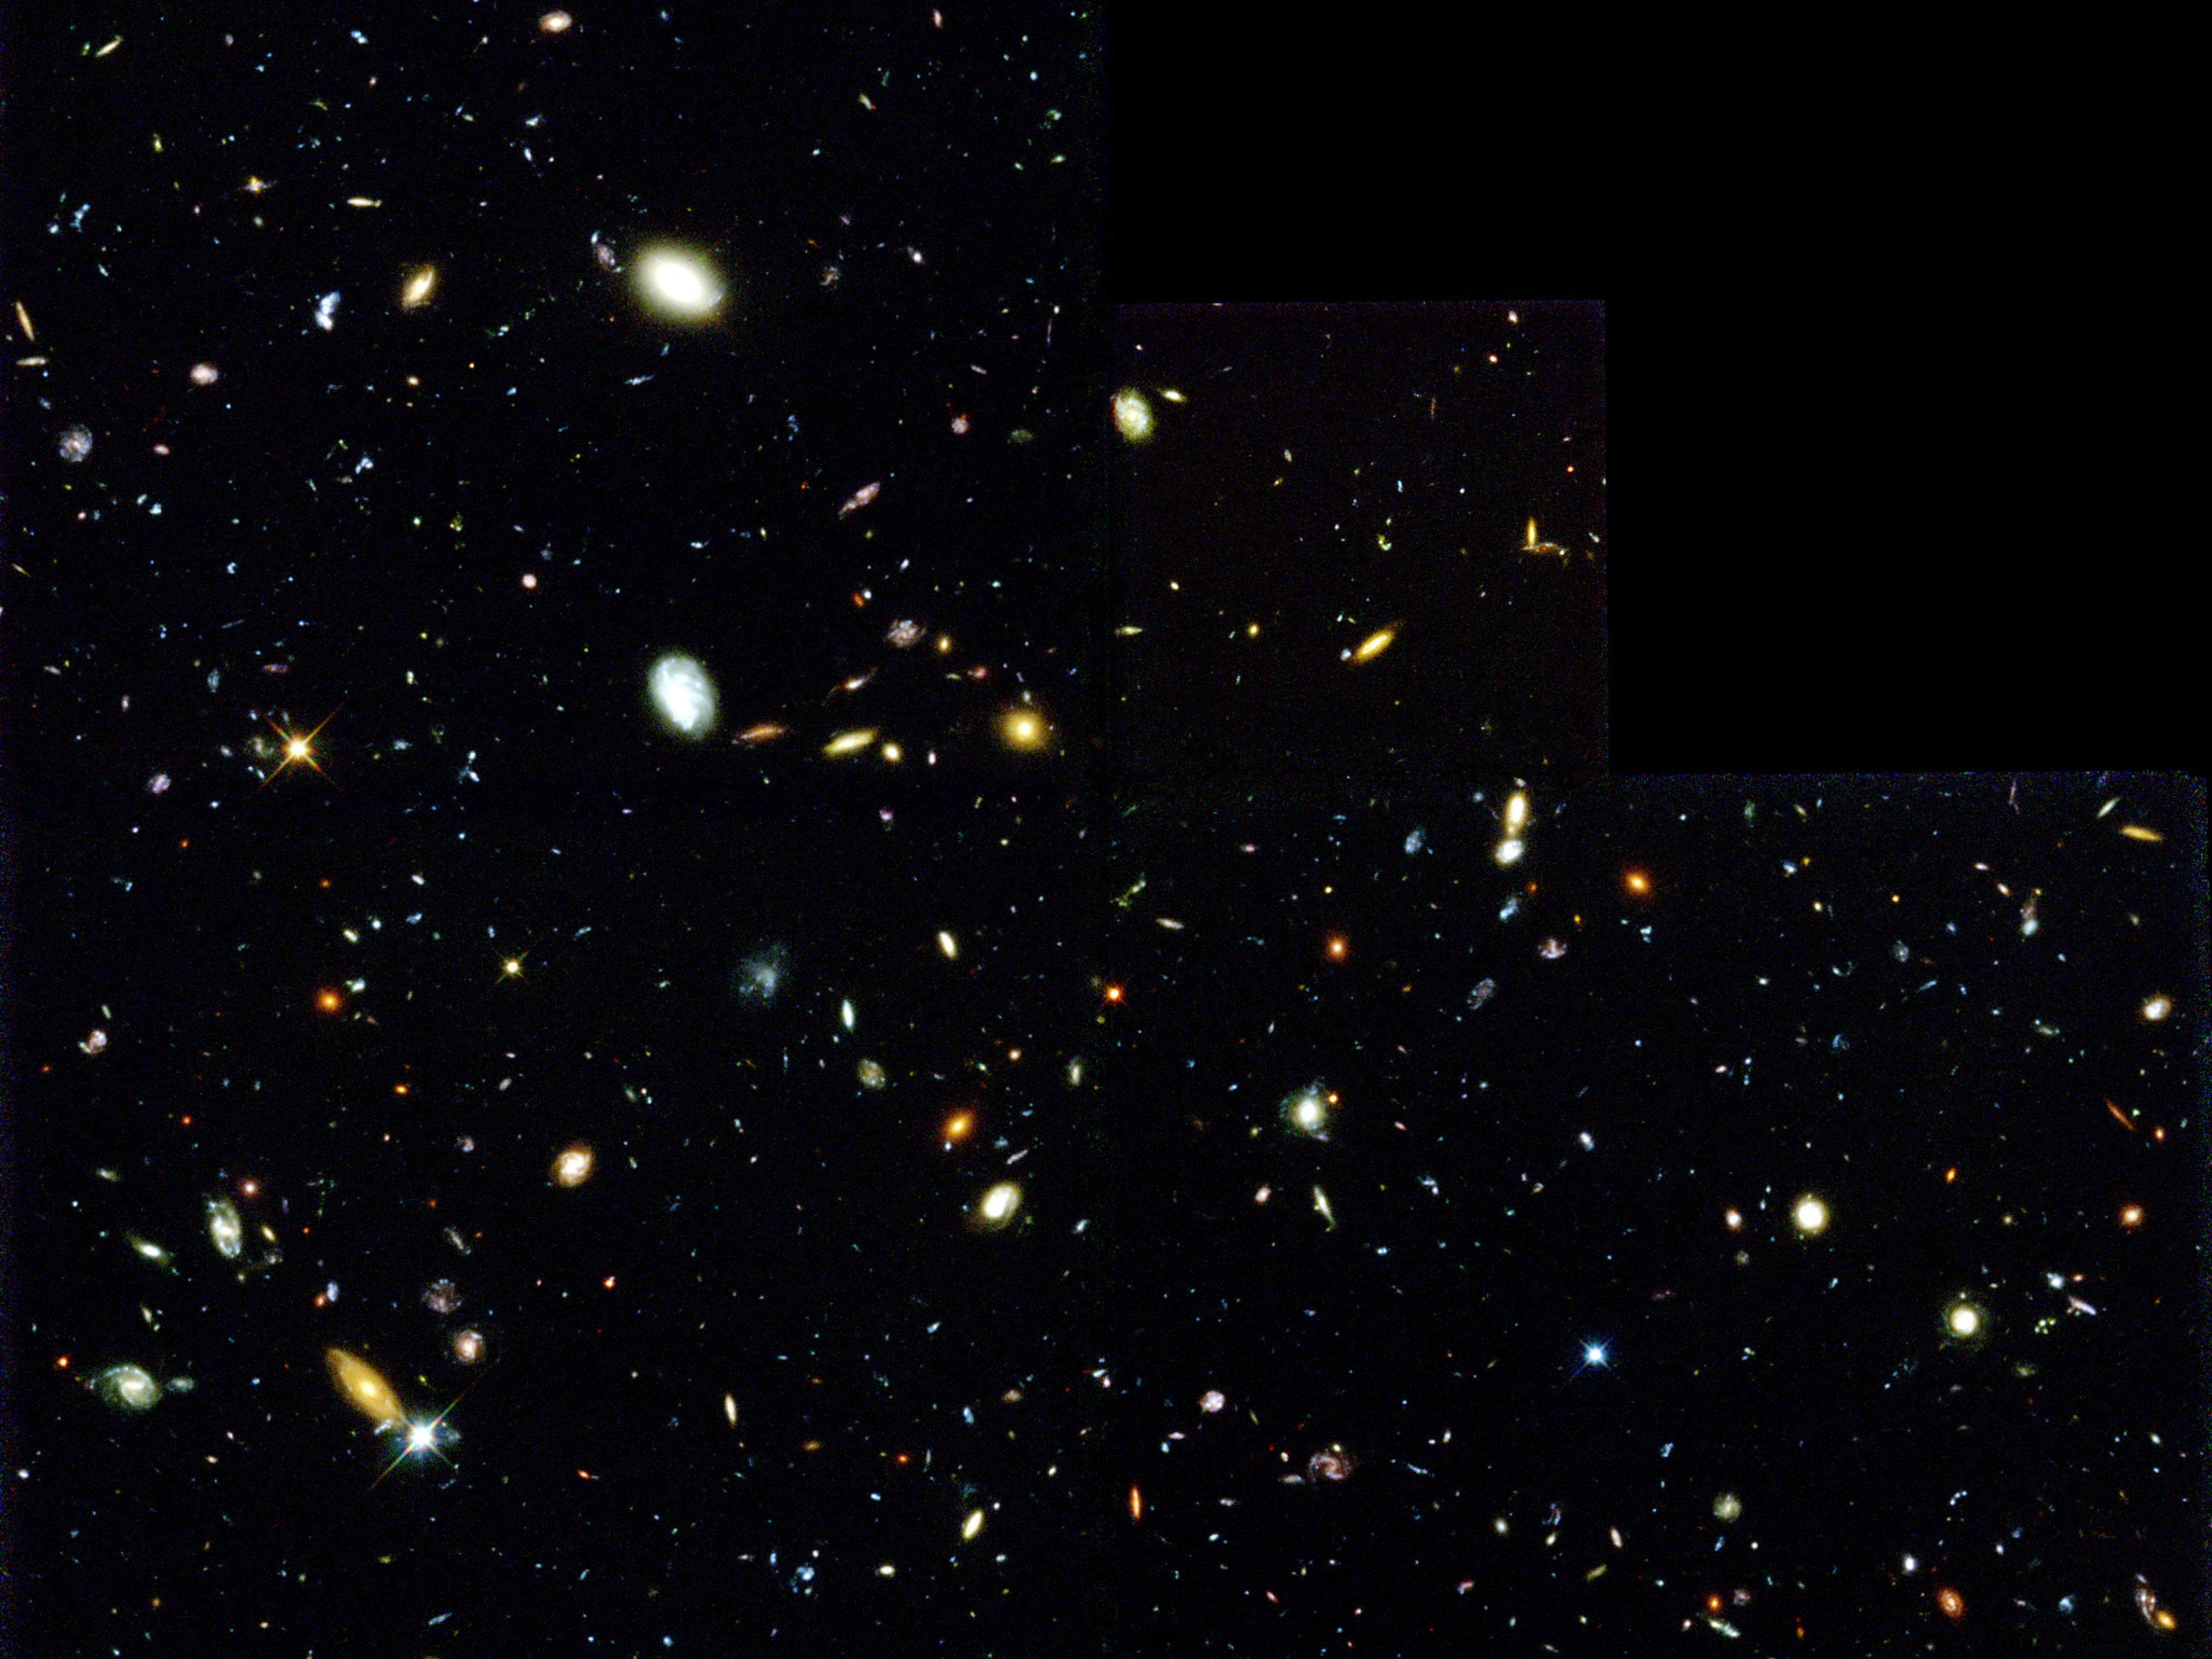
\includegraphics[width=0.9\columnwidth]{Figures/hubble_deep_field.pdf}
	\caption{The Hubble Deep Field as captured by the Wide Field and Planetary Camera 2 onboard the \textit{Hubble Space Telescope} in 1995.}
	\label{fig:hubble_deep_field}
\end{figure}

\section{Galaxy Formation and Evolution}

To answer our questions on the evolution of galaxies, we must first make some inferences about the {\color{red}[...]} of the Universe. Our understanding of the cosmic history of galaxies is dependent on our choice of cosmology, which is widely accepted to be in the form of the $\Lambda$-CDM model (\citealt{Peebles_1980}). In the $\Lambda$-CDM model, Cold Dark Matter, matter of unknown origin, dominates over ordinary baryonic matter; and with dark energy, constitute a combined $\sim 95\%$ of the total cosmic energy budget (\citealt{Fukugita_2004}). The presence of dark matter is only evident in its gravitational interactions with other matter, but its origin is unknown as it does not interact with nor emit any electromagnetic radiation. The dark energy in the Universe is parameterized in the form of the cosmological constant, $\Lambda$, which is required to explain the accelerating expansion of the Universe. In this model, galaxy formation is seeded by small quantum fluctuations in the density of the early Universe, which grow with inflation to form small overdensities that later become the sites of dark matter halos by gravitationally attracting nearby dark matter. The first galaxies formed from these originally minute overdensities in density, which later merge due to an increase in collisions in a smaller Universe, to form ever larger galaxies. This model of galaxy formation is called a 'hierarchical' model, where galaxies in the early Universe are expected to be smaller and formed their mass more quickly than massive galaxies at later times that formed much of their stellar mass from previous mergers. As we shall show in Chapter \ref{chapter:Radio_Identifications}, this model of evolution may not explain the stellar build up of all galaxies.

\subsection{Classification of Galaxies}

The first step in understanding galaxy evolution by observing how galaxies have changed as we look back in time, is to classify galaxies according to their observable properties. Generally, galaxies can be classified into two broad groups based on their morphology: spirals and ellipticals. This dichotomy prompted the first classification scheme by Edwin Hubble (Figure \ref{fig:hubble_tuning_fork}; \citealt{Hubble_1936}), the \textit{Tuning Fork}, which shows ellitpical galaxies along the "handle", becoming more oblate towards the spiral galaxies. The spiral galaxies themselves are split into two categories forming the two "prongs", depending on the presence of a bar at the centre. At the join of the two, classified on the \textit{Tuning Fork} as S0, is where we might locate \textit{lenticular galaxies}, that are recognized by their large disks, like spirals, but without the presence of arms. In the rest of this Thesis we shall predominantly be referring to elliptical galaxies at \textit{early-type galaxies} (ETGs) and spiral-like galaxies as \textit{late-type galaxies} (LTGs), as is convention. Despite their names, the two do not represent a former and latter evolutionary stage of a typical galaxy, and is rather a misnomer. A minority of galaxies do not conform to this dichotomous image and are typically grouped together as \textit{irregular galaxies}.

\begin{figure}
    \centering
	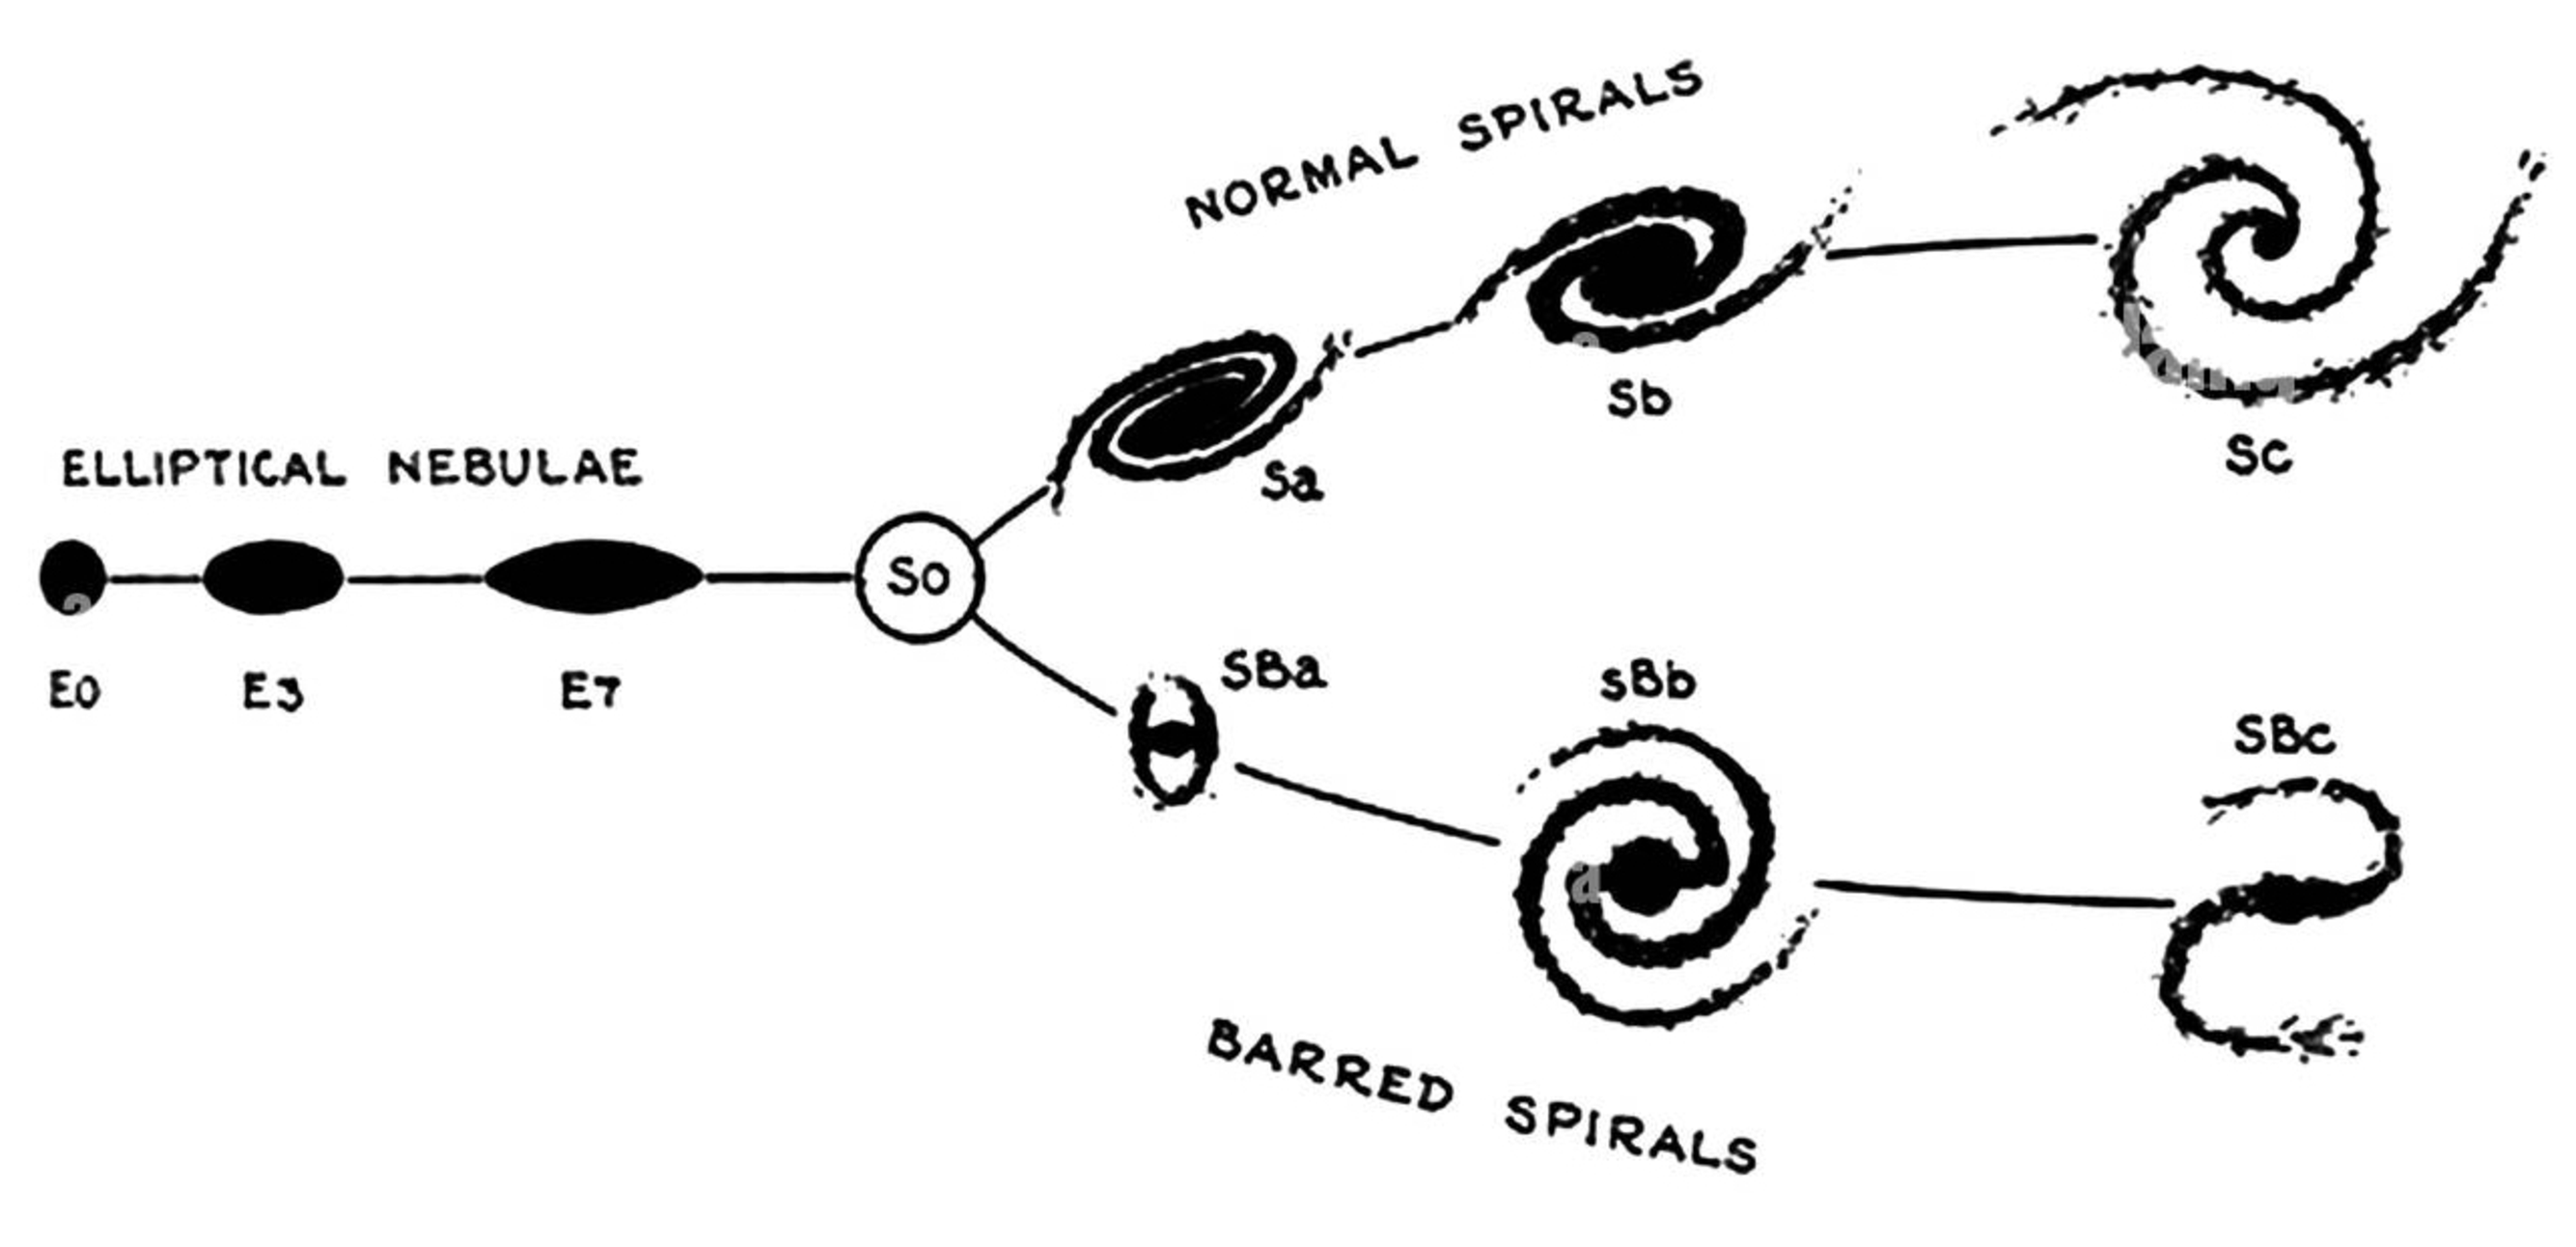
\includegraphics[width=0.9\columnwidth]{Figures/hubble_tuning_fork.pdf}
	\caption{The \textit{Hubble Tuning Fork}, or the \textit{Sequence of Nebular Types} as named in \citealt{Hubble_1936}, showing spiral galaxies along the prongs of the tuning fork and elliptical galaxies along the handle. The two prongs separate those spiral galaxies with barred central bulges from those that do not. Lenticular galaxies can be found at the join of the handle to the prongs. From left to right, the elliptical galaxies become more oblate and the spiral galaxies have spiral arms that become less tightly wound around the central bulge.}
	\label{fig:hubble_tuning_fork}
\end{figure}

Beyond their shape, the two broad groups, ETGs and LTGs, have a number of physical characteristics that are common to galaxies of the same class. First, the stellar populations of ETGs and LTGs are different. ETGs are dominated by old stellar populations that appear red in colour because they contain longer-lived, low mass stars, whereas LTGs typically have younger stellar populations of massive, but very short-lived stars.

ETGs are considered to be some of the most massive, luminous galaxies (due to having vast quantities of old stars) observed in the local Universe (\citealt{Bernardi_2003}; \citealt{Kelvin_2014}; \citealt{Moffett_2016}). Their stellar content is often centrally distributed, with the density of stars decreasing to the outskirts of the galaxy. In this central bulge of stars is where most of the interstellar medium (ISM) is located, though it is not expected to be substantial, and the limited amount of gas prohibits new star formation. In a hierarchical view of star formation, such ellipticals are formed from a series of major and minor mergers that consume the gas in the galaxy, leading to the quiescent systems observed today (\citealt{Toomre_1972}). In contrast, LTGs have dusty spiral arms with sites of active star formation, with older stars mainly located within the central bulge. While ETGs are largely devoid of gas, LTGs have a rich ISM that continues to fuel star formation, creating new stars at typical rates of several stars per year (\citealt{Kennicutt_1983}; \citealt{Gao_2004}). Our own Milky Way is an SBc spiral galaxy (\citealt{Gerhard_2002}) with active star formation at a rate of $\sim 2\,M_\odot$yr$^{-1}$ (\citealt{Noriega-Crespo_2013}; \citealt{Licquia_2015}; \citealt{Elia_2022} and references therein).

\subsection{The Star Forming Main Sequence}

A natural diagram to illustrate the difference in colour of ETGs and LTGs is to show the colours of optically-selected galaxies against their absolute magnitude. Galaxies discovered in optical surveys readily form two distinct regions: a \textit{red sequence} and a \textit{blue cloud}, with a sparsely populated region in between, the \textit{green valley}. Due to their optical colours, the red sequence is dominated by ETGs and the blue cloud dominated by LTGs. Moving away from observed quantities to intrinsic quantities, we note that the colour is a strong indicator of the star formation rate (SFR) in a galaxy and that absolute magnitude is approximately proportional to the size of the stellar population, and thus the stellar mass, $M_*$. In this formalism, the blue galaxies form a tight correlation known as the \textit{Main Sequence} (MS) or \textit{Star Forming Main Sequence}, while the red sequence occupies a \textit{passive cloud} (or "red and dead" or "quiescent") region that lies below the MS at lower star formation rates (\citealt{Noeske_2007}; \citealt{Daddi_2007}; \citealt{Elbaz_2007}; \citealt{Rodighiero_2011}). Figure \ref{fig:star_forming_main_sequence} shows the main sequence and passive clouds (grey contours) that form from the optically-selected Sloan Digital Sky Survey (SDSS; \citealt{York_2000}). \citealt{Saintonge_2017} present the \textit{Extended CO Legacy Database for GASS}, xCOLD GASS, a mass-selected sample from SDSS that have molecular gas mass estimates, which are plotted in colour in Figure \ref{fig:star_forming_main_sequence}. The molecular gas mass fraction, $f_{\textrm{H}_2} \equiv M_{\textrm{H}_2}/M_*$, clearly declines towards the passive cloud, showing the depleted ISM in ETGs.

{\color{red}Perhaps add a paragraph on the stellar-mass growth sequence, as illustrated by Figure 12 of Graham+2023}

\begin{figure}
    \centering
	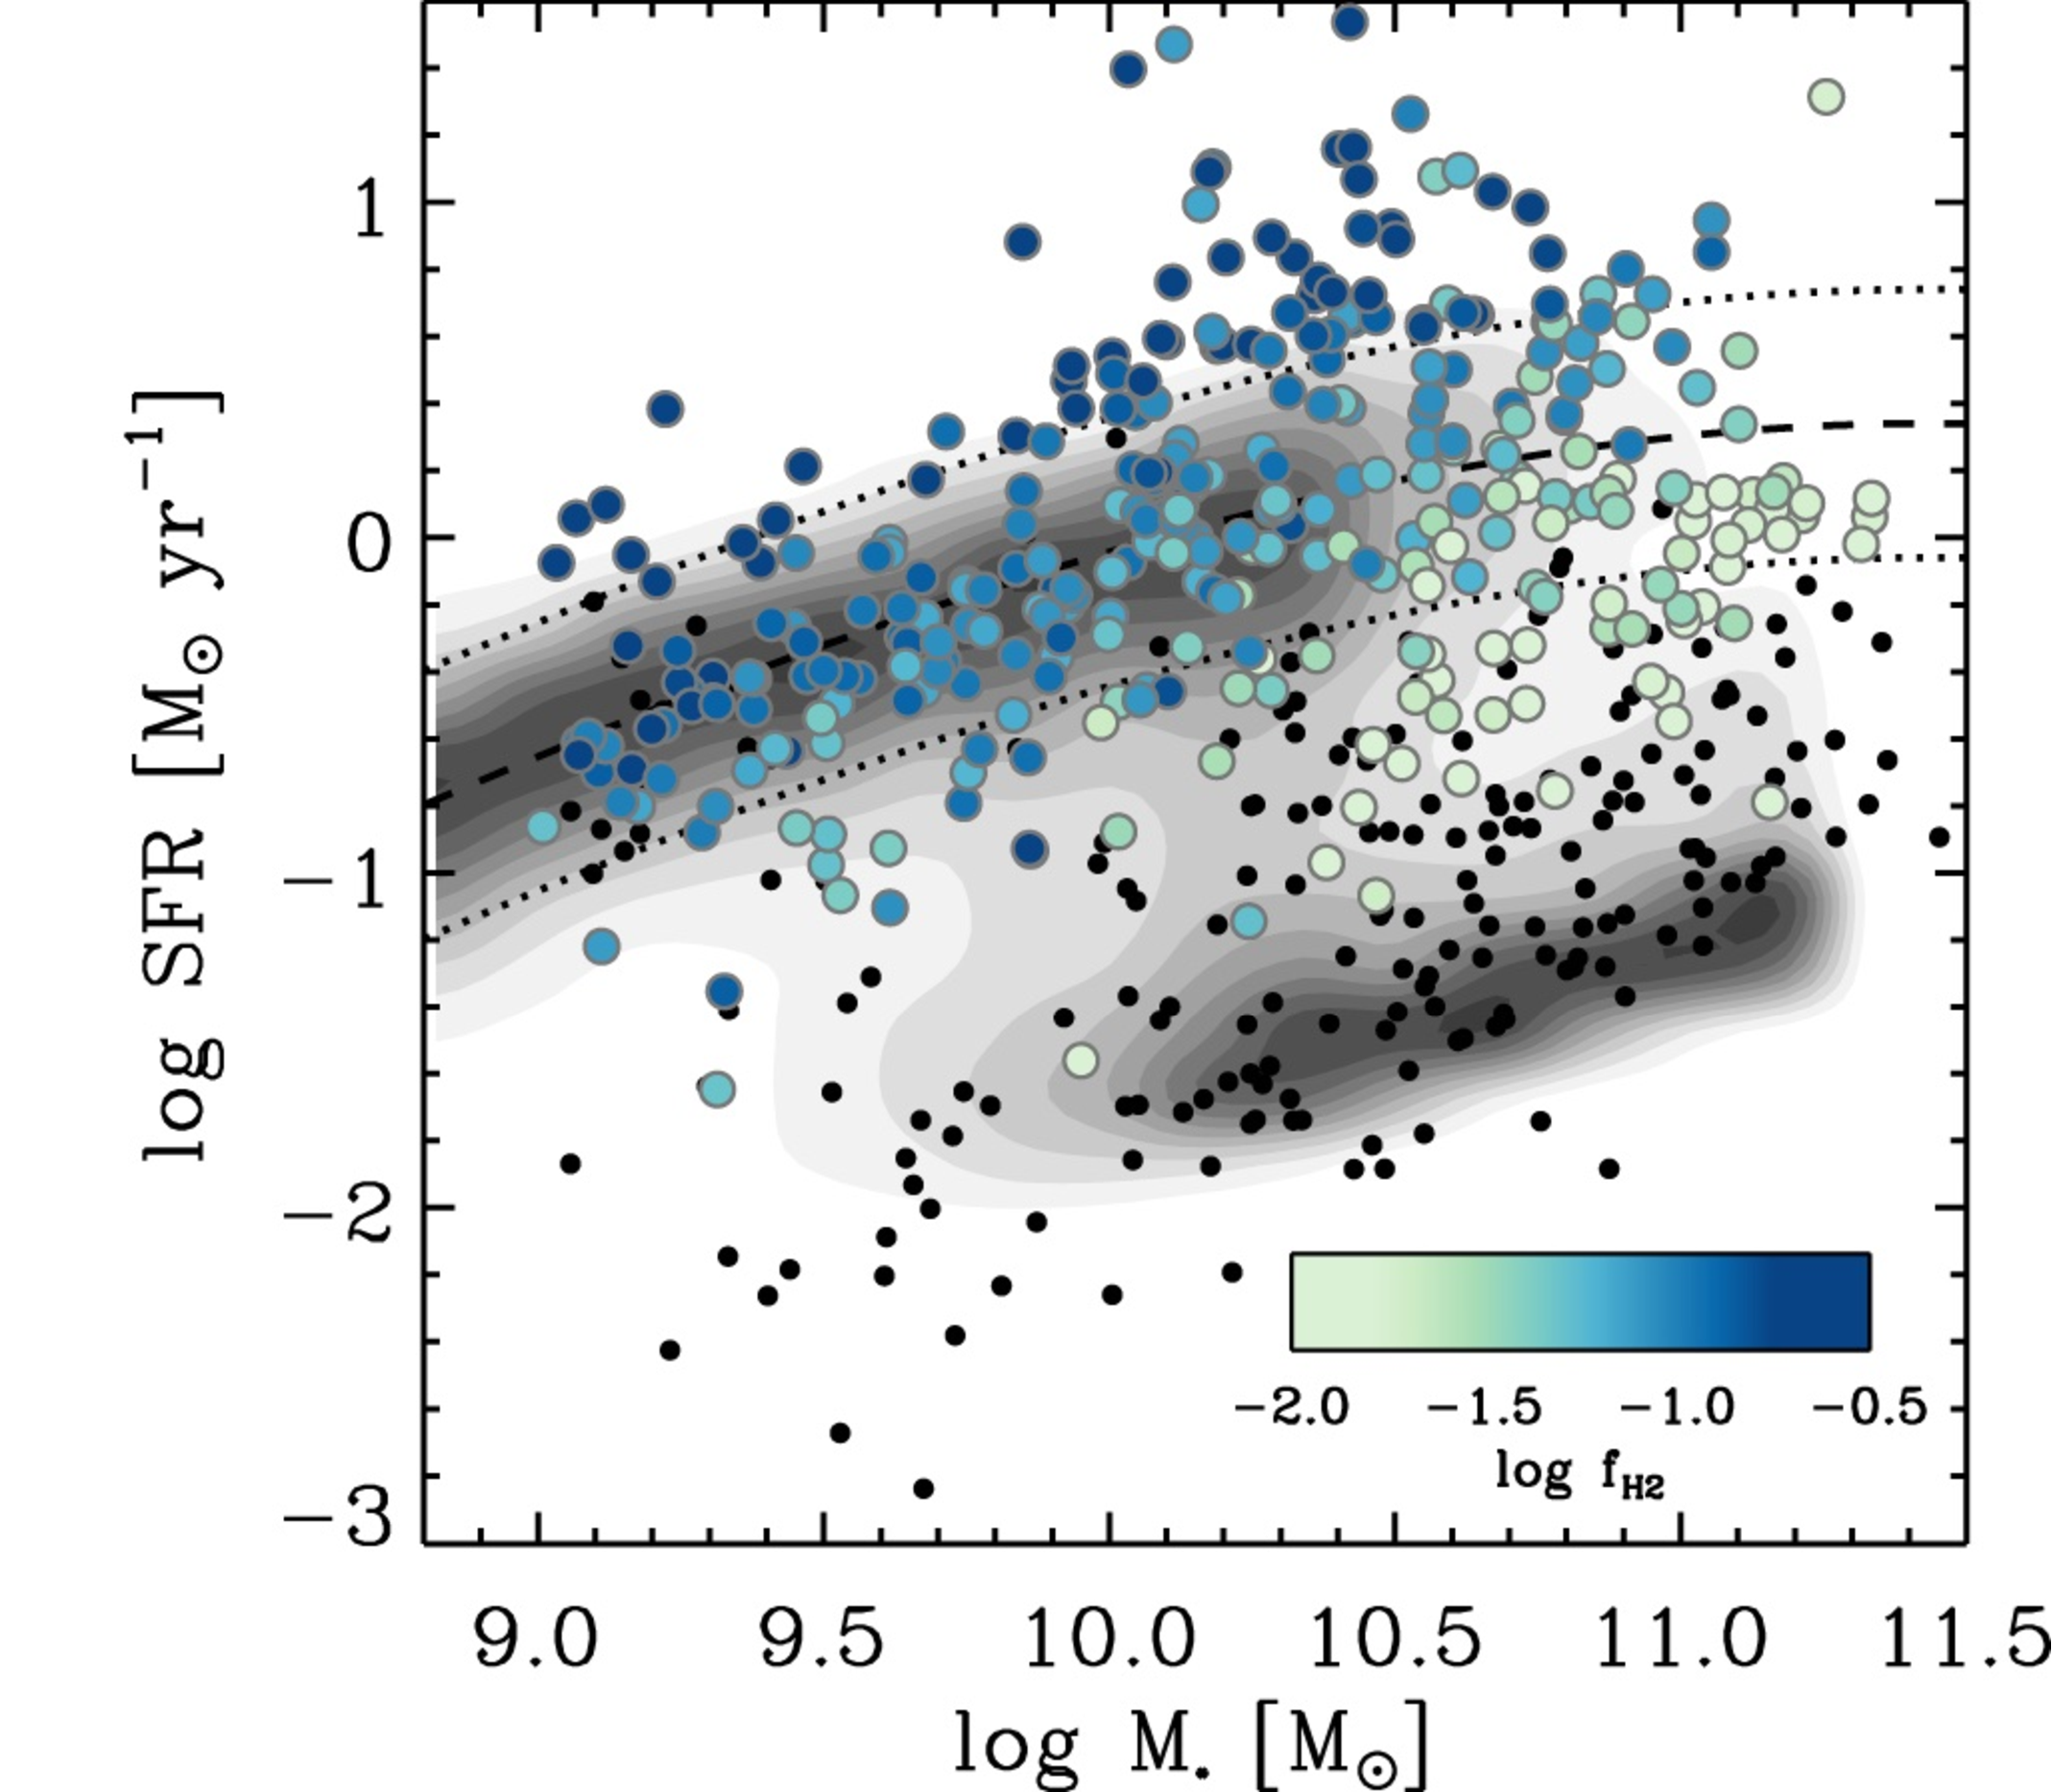
\includegraphics[width=0.75\columnwidth]{Figures/saintonge_ms.pdf}
	\caption{The distribution of SDSS galaxies in the SFR-$M_*$ plane (grey contours) from \citealt{Saintonge_2017} (Figure 7). The dashed line represents the location of the main sequence, while the dotted lines represent $\pm0.4\,$dex scatter around this relation. The coloured points show the distribution of galaxies from xCOLD GASS, coloured according to their molecular gas mass fraction.}
	\label{fig:star_forming_main_sequence}
\end{figure}

It is predicted that the vast majority, approximately $90\%$, of all cosmic star formation between redshifts $0$ and $2.5$ occurs in galaxies that reside on the MS, however, an important contribution also comes from galaxies that sit substantially above the relation. These galaxies, undergoing high levels of star formation for a short period of time, are collectively referred to as \textit{starburst galaxies} (e.g. \citealt{Muxlow_2006}; \citealt{Rinaldi_2022}). Starbursts form a small minority of galaxies, approximately $2\%$ of star forming galaxies depending on the exact definition of a starburst, but contribute $\sim 10\%$ of the cosmic star formation rate density (SFRD) at $z \sim 2$ (\citealt{Rodighiero_2011}), corresponding to the time in cosmic history when star formation was at its peak (see Section \ref{sec:cosmic_star_formation_history}).

Given that galaxies in the passive cloud have large stellar masses, they must have been at some point among the actively star forming galaxies, and then some process quench them of their star formation leading them to the passive cloud. The prevailing interpretation of the SFR-$M_*$ diagram is that a typical galaxy evolves along the sequence, gaining stellar mass, increasing their star formation rate accordingly and depleting the gas available for star formation in the process. At some point, the galaxy stops forming stars entirely, and falls off the main sequence. The valley between the MS and the passive cloud, a result of a dearth of galaxies in this regime, suggests that the quenching process that turns off the star formation in the galaxy is fast. This image of galaxy evolution, however, is not without scepticism. Recent studies (e.g. \citealt{Eales_2018}; \citealt{Bremer_2018}; \citealt{Phillipps_2019}) have suggested that the bimodal distribution of star forming and passive galaxies may be a reflection of selection effects in optical surveys, prompting attempts to define the whole population of galaxies using a probability distribution with only one maximum (e.g. \citealt{Corcho-Caballero_2020}). {\color{red}Explain the evidence for an apparent bimodality (Read abstracts of three papers above - that is all that is needed.)}

Whether there are two distinct classes or whether the transition between morphological types and physical properties is gradual, some physical process must be coverting a star forming galaxy on the MS to one that is passive, quenching it of star formation. There are many possibilities that have been proposed as the cause of quenching, and it is likely that all are important in different scenarios. These processes include stellar feedback and winds from supernovae removing the gas from a galaxy (\citealt{Hayward_2017}); gas expulsion by active galactic nuclei, AGN (\citealt{Springel_2005}; \citealt{Croton_2006}; \citealt{Cicone_2014}; \citealt{Harrison_2017}); the formation of a galactic bar or central bulge (\citealt{Bournaud_2007}; \citealt{Martig_2009}) which relocates the gas to the galactic center and reduces the star formation in the disk, as well as a range of environmental processes such as galaxy merging (\citealt{Lavery_1994}; \citealt{Weigel_2017}) which ignites a starbursting phase that rapidly consumes the gas; ram-pressure stripping, the loss of gas as the galaxy passes through the intra-cluster medium (\citealt{Gunn_1972}; \citealt{Boselli_2006}; \citealt{Domainko_2006}; \citealt{Boselli_2014}), and quenching mechanisms that result from being in high density environments such as galaxy clusters, like galaxy harassment and strangulation (\citealt{Moore_1996}; \citealt{Moore_1998}; \citealt{Bekki_2002}).

\subsection{Cosmic Star Formation History}
\label{sec:cosmic_star_formation_history}

We have seen that the star formation rates of galaxies is intrinsically linked to its evolutionary stage, and thus it would be unsurprising to identify an evolution in the integrated SFRs of galaxies with cosmic time. By measuring the star formation of many galaxies at different epochs, we can build a picture of the star formation density in the Universe. The cosmic history of star formation is one of the fundamental observables of astronomy, giving us an insight into the timeline for which gas forms into stars, heavy elements are produced (elements heavier than the primordial hydrogen and helium are produced in stars), and dust is formed (as dust is a natural byproduct of star formation, see Section {\color{red}X}).

The cosmic star formation rate density (SFRD {\color{red}Repeated}) in the Universe can be estimated in two ways. The most straightforward way to estimate the star formation rate is to measure the amount of starlight we observe from tracers of recent star formation in galaxies. In this sense, the SFR indicator should be sensitive to the short-lived massive stars at each point in cosmic history, and thus the UV and optical stellar light is often used (e.g. \citealt{Madau_1996}; \citealt{Lilly_1996}; \citealt{Wyder_2005}; \citealt{Schiminovich_2005}; \citealt{Dahlen_2007}; \citealt{Reddy_2009}; \citealt{Robotham_2011}; \citealt{Cucciati_2012}; \citealt{Schenker_2013}; \citealt{Finkelstein_2015}). Second, we note that approximately half of all optical and UV light from stars ever emitted in the Universe has been absorbed by dust and re-emitted at far-infrared (FIR) and sub-millimeter (sub-mm) wavelengths (\citealt{Puget_1996}; \citealt{Fixsen_1998}; \citealt{Dole_2006}; \citealt{Driver_2008}; \citealt{Driver_2016}). This means that a significant contribution to the SFRD must also be measured from far-IR/sub-mm indicators of star formation that probe the stellar light reprocessed by dust (e.g. \citealt{Magnelli_2011}; \citealt{Casey_2012}; \citealt{Magnelli_2013}; \citealt{Gruppioni_2013}; \citealt{Swinbank_2014}; \citealt{Bouwens_2016}; \citealt{Bourne_2017}; \citealt{Koprowski_2017}; \citealt{Novak_2017}; \citealt{Liu_2018}; \citealt{Bouwens_2020}; \citealt{Dudzeviciute_2020}).

{\color{red}Rewrite above as it is not strictly two separate ways. See Wise+2023.}

Figure \ref{fig:cosmic_sfrd} shows that the dust-obscured and unobscured measures of the SFRD have peaks at $z\sim2$ (when the Universe was roughly 3 billion years old), followed by a slow decline by a factor of $\sim 8$ to the present day. The short period corresponding to the peak of star formation is often referred to as \textit{cosmic noon}. In the (approximate) 3.5\,Gyr between $z\sim3$ and $z\sim1$, spanning cosmic noon, up to half of the stellar mass we observe today was formed (\citealt{Forster-Schreiber_2020}). The galaxies that are identified at these redshifts are ideal targets for tracing the formational epoch of the massive LTGs and ETGs seen in the local Universe. We see that most of the star formation at $z < 3$ is obscured by dust and even at higher redshifts the contribution appears significant. The FIR and sub-mm traced component has dominated the cosmic history of star formation for the past $\sim 12\,$Gyr, contributing approximately $80\%$ of the total star formation. The top panel of Figure \ref{fig:cosmic_sfrd} shows the contribution from galaxies with different IR luminosities to the dust-obscured star formation. It is clear that massive, IR luminous galaxies dominate the star formation history at earlier times. At this point, we clarify some acronynms commonly used to refer to bright infrared galaxies (the IR luminosities of galaxies are assumed to be the bolometric luminosity integrated between $8$ and $1,000\,\mu$m):

\begin{itemize}
    \item Luminous Infrared Galaxy (LIRG) - Defined as having $10^{11} < L_\textrm{IR} [L_\odot] < 10^{12}$.
    \item UltraLuminous Infrared Galaxy (ULIRG) - Defined as having $10^{12} < L_\textrm{IR} [L_\odot] < 10^{13}$.
    \item HyperLuminous Infrared Galaxy (HyLIRG) - Defined as having $L_\textrm{IR} [L_\odot] > 10^{13}$.
\end{itemize}

\begin{figure}
    \centering
	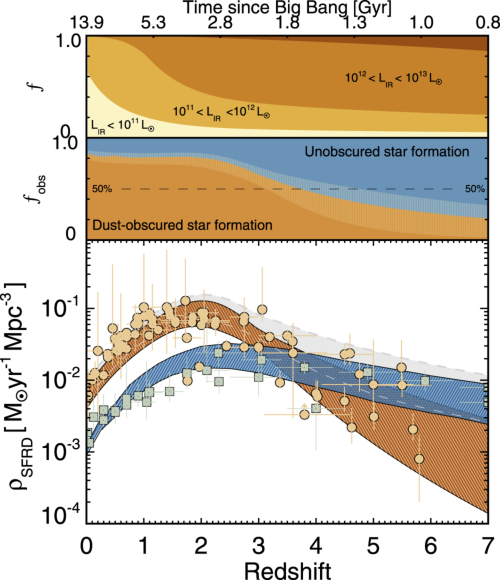
\includegraphics[width=0.75\columnwidth]{Figures/cosmic_sfrd.pdf}
	\caption{The cosmic star formation history from \citealt{Zavala_2021}. The contributions to the total star formation rate density (grey) from dust-obscured IR/sub-mm surveys and from unobscured UV/optical surveys are shown in orange and blue, respectively. The top panel shows the contribution from galaxies with different IR luminosities to the dust-obscured SFRD. The classes shown are $L_\textrm{IR} < 10^{11}\,L_\odot$, $10^{11} < L_\textrm{IR} [L_\odot] < 10^{12}$ (LIRGs) and $10^{12} < L_\textrm{IR} [L_\odot] < 10^{13}$ (ULIRGs). The middle panel represents the fraction of SFRD that is dust-obscured.}
	\label{fig:cosmic_sfrd}
\end{figure}

Looking back to cosmic noon, much of the star formation within dusty galaxies is happening in ULIRGs, while the integrated dust-obscured star formation begins to fall. This suggests that the number of massive galaxies declines at higher redshifts. Particularly at high redshifts ($z \gtrsim 3$), the exact amount of dust-obscured star formation is still uncertain. Large samples of galaxies with measured dust emssion are therefore required to elucidate our view on the cosmic history of star formation.

\section{The Interstellar Medium}

The interstellar medium (ISM) refers to the matter that fills the space in between the stars of a galaxy. It is the medium in which stars are born, and latter replenished with enriched material when they die. The matter comes in the form of gas - in ionic, atomic and molecular forms - and dust, in overwhelming favour of gas which constitutes $\sim99\%$ of the ISM, and dust the other $1\%$ ({\color{red}REFERENCE}). By mass, the gas in the ISM is around $70\%$ hydrogen, $28\%$ helium and $2\%$ heavier elements, reflecting only a small change from the ratios of the primordial matter created after the Big Bang (\citealt{Klessen_2016}). In terms of volume, most of the ISM is occupied by ionized gas, but due to its incredibly low volume density, only accounts for around $25\%$ of the gas mass. Most of the gas mass in a galaxy is in the form of neutral atomic gas (H and He) or molecular (H$_2$) and can be found in dense clouds that take up only $1-2\%$ of the total volume of the ISM.

The ISM spans a wide range of temperatures and densities, leading to many interpretations of the ISM as being in distinct phases, despite there being no obvious separation between different phases (\citealt{Cox_2005}). A two phase model was proposed by \citealt{Field_1969}, showing that atomic gas in the ISM can exist at two stable temperatures. These two solutions correspond to cold and dense gas at $T\sim100\,$K and warm, diffuse gas at $T\sim10^4\,$K. These are now referred to as the Cold Neutral Medium (CNM) and Warm Neutral Medium (WNM), respectively. This model was extended to three phases by \citealt{McKee_1977}, who noted that supernovae in the ISM creates bubbles of very hot, ionized gas ($T\sim10^6\,$K). This phase of the ISM is known as the Hot Ionized Medium (HIM). A cooler, Warm Ionized Medium (WIM) has a temperature and density similar to the WNM, but contains around $90\%$ of the ionized gas in the ISM (\citealt{Haffner_2009}). A final distinction is typically made for the molecular clouds that are cold, but distinctly more dense than the CNM. The molecular gas clouds have a range of masses and sizes, and is known to correlate with observed star formation in the Galaxy. The approximate temperatures, densities, mass fractions and volume filling fractions of the phases in the ISM for a dynamic spiral galaxy is given in Table \ref{tab:ISM_phases} as presented in \citealt{Ferriere_2001} and {\color{red}Walter?}. The fractions are highly uncertain but represent what might be realistic estimates for a spiral galaxy containing all five phases of this model of the ISM.

\begin{table}
	\centering
	\begin{tabular}{p{4cm}|p{3cm}|p{3cm}|p{1.5cm}|p{1.5cm}}
		\hline
		\hline
		Phase & T [K] & $n$ [atoms cm$^{-3}$] & $f_{\textrm{Mass}}$ & $f_{\textrm{Volume}}$ \\
		\hline
		\hline
		Molecular Clouds & $10 - 20$ & $>10^2$ & $\sim 20\%$ & $<1\%$ \\
		Cold Neutral Medium & $50 - 100$ & $20 - 50$ & $\sim 40\%$ & $\sim2 - 4 \%$\\
		Warm Neutral Medium & $6,000 - 10,000$ & $0.2 - 0.5$ & $\sim 30\%$ & $\gtrsim 30\%$ \\
		Warm Ionized Medium & $\sim8,000$ & $0.2 - 0.5$ & $\sim 10\%$ & $\gtrsim 15\%$ \\
		Hot Ionized Medium & $\sim10^6$ & $\sim10^{-2}$ & $\sim 1\%$ & $\lesssim 50\%$ \\
		\hline
	\end{tabular}
	\caption{The different phases of the ISM and their expected temperatures, densities, mass fractions and volume filling factors.}
	\label{tab:ISM_phases}
\end{table}

This multi-phase picture is certainly an oversimplification of the conditions found in the ISM. The ISM is shaped by a variety of processes that blur the distinction between these distinct phases. The actual ISM is continuous and dynamic with transitional regions between the phases. Processes that contribute to the blurring of the boundaries between different phases include turbulence from supernova shocks (\citealt{MacLow_2004}) and stellar winds, thermal instability (\citealt{Kritsuk_2002}) and the presence of magnetic fields.

Figure \ref{fig:interstellar_medium} shows various components of the ISM in the Galaxy, as traced by different wavelengths of the electromagnetic spectrum. The top two panels highlight the starlight that is observable at optical ($0.5\,\mu$m) and near-infrared ($2\,\mu$m) wavelengths. The stellar light is blocked by dust in the optical image, whereas the near-infrared clearly shows the stellar distribution, making the dark dust clouds appear almost transparent. The benefit that the infrared provides in identifying the stellar light of a galaxy, compared to optical wavelengths, is a key motive for the studies presented in Chapters \ref{chapter:Data_Release_3} and \ref{chapter:Dust_Mass_Functions}. As we traverse the electromagnetic spectrum to the far-infrared (third panel, observed at $350\,\mu$m) the emission from the dust itself becomes visible. The final three panels show the emission from atomic, ionized and molecular gas in the Galaxy. The atomic gas is traced by the $21\,$cm spectral line, originating from the hydrogen \textit{spin-flip} transition between a proton-electron aligned state to an anti-aligned state. This transition is forbidden - the mean lifetime of a hydrogen atom being in the excited, aligned state is approximately 11 million years ({\color{red}REFERENCE}) - meaning that the likelihood of the transition is incredibly rare. However, as can be seen in the figure, the abundance of atomic hydrogen means that the $21\,$cm line is a useful tracer for gas in the ISM. The limitation of the $21\,$cm line is that it is only useful for tracing the distribution of neutral hydrogen in the local Universe where the emission is still strong enough to be detected. The $74\,$cm radio emission in the penultimate panel traces the radiation from ionized gas. The radio emission emanates from accelerated charged particles, which may be observed in HII regions and supernova remnants. The final panel shows the molecular gas phase, as traced by the $2.6\,$mm spectral line of carbon monoxide (CO). As will be detailed later, the rotational transitions of the CO molecule is a useful tracer of dense molecular regions, and it is often assumed that wherever there are CO molecules there must also exist H$_2$ molecules. This map shows the locations of cold gas in the Galaxy and the sites of star formation.

\begin{figure}
    \centering
	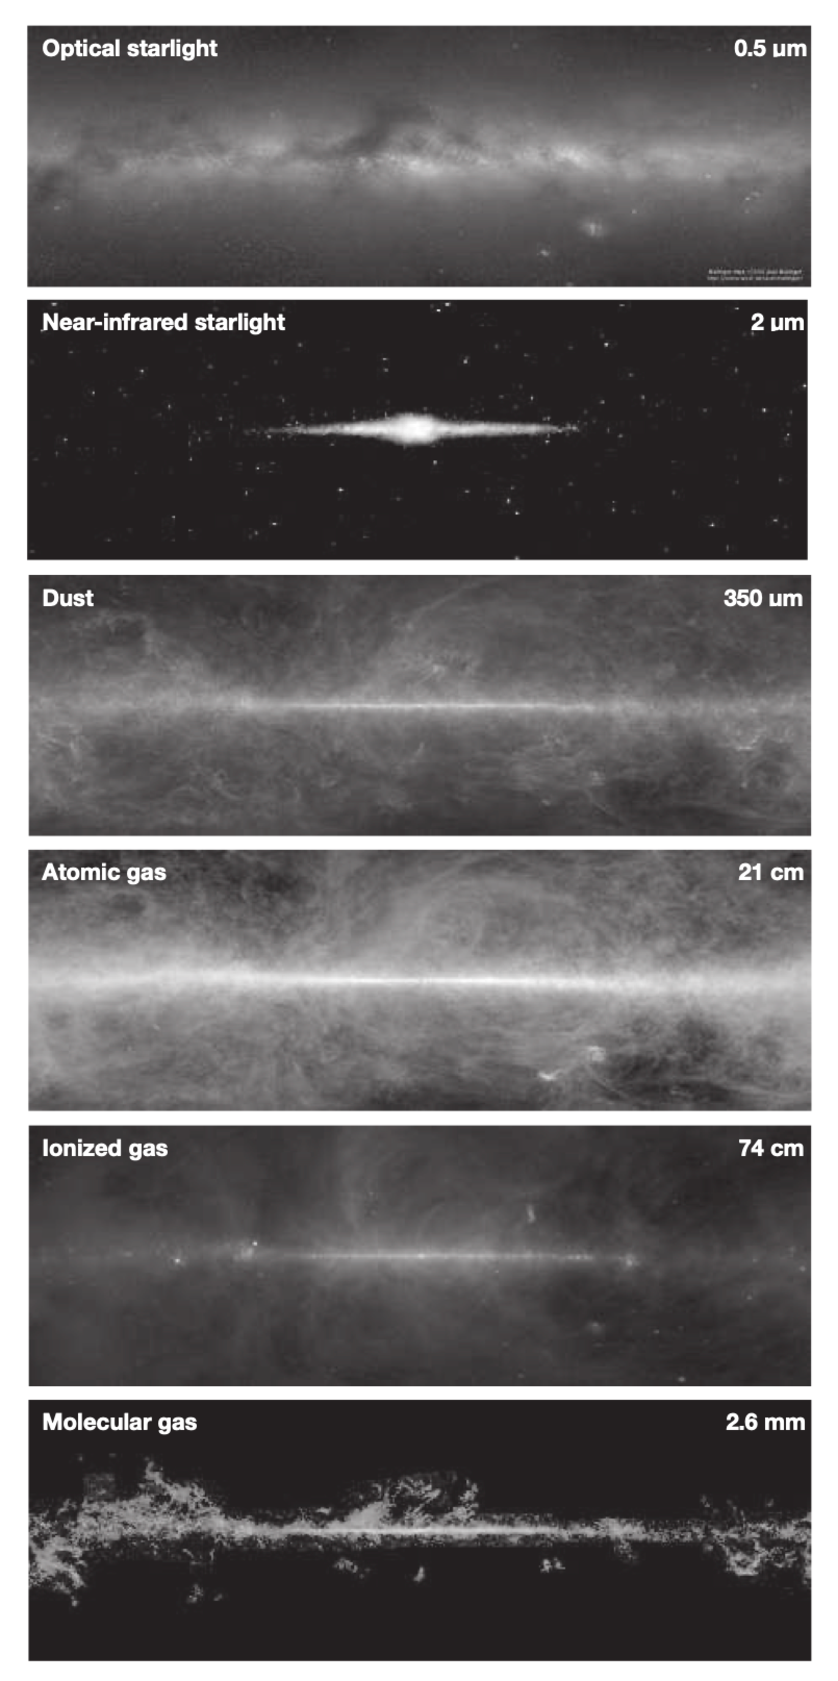
\includegraphics[width=0.75\columnwidth, height=0.92\textheight]{Figures/interstellar_medium.pdf}
	\caption{The plane of the Galaxy observed at different wavelengths as presented in \citealt{Williams_2021}. From top to bottom the panels show: the optical starlight at $0.5\,\mu$m; the near-infrared starlight at $2\,\mu$m; the interstellar dust at $350\,\mu$m; the atomic gas at $21\,$cm; the ionized gas at $74\,$cm and the molecular gas at $2.6\,$mm.}
	\label{fig:interstellar_medium}
\end{figure}

\section{Cosmic Dust}

\subsection{Chemical Composition of Dust}

Cosmic dust is a general term that refers to the solid particles that exist in the ISM. These interstellar grains can have a range of sizes between $\sim 10\,$nm and $\sim 1\,\mu$m (\citealt{Kim_1994}; \citealt{Galliano_2018}) and are mostly composed of carbonaceous materials (materials that are predominantly Carbon by mass) and silicates. The larger dust grains are primarily silicates and amorphous carbon, which are the prime candidates for the dust grains that absorb UV and optical starlight and reradiates this energy in the far-IR and sub-mm regimes. Hydrogenated carbonaceous materials, like Polycyclic Aromatic Hydrocarbons (PAHs), are chemical compounds comprised of carbon and hydrogen molecules and are also {\color{red}[...]} interstellar dust grains. These molecules are the cause of strong spectral lines that can be observed in the mid-infrared (\citealt{Tielens_1987}; \citealt{Draine_2007a}; \citealt{Draine_2007b}).

\subsection{The Reprocessing of Starlight}

The presence of dust along the line of sight to a population of stars can have several consequences on the emission that is observed. First, if the dust is thick enough, any background stellar light may not be visible at all, as is the case with some dark nebulae in the Galaxy such as the \textit{Horsehead Nebula}. For less opaque dust clouds, the light passing through can be dimmed due to the effects of dust extinction. This refers to the amount of background light that is absorbed and scattered out of the line of sight to the observer. The dimming effect is dependent on several factors including the density of the dust cloud, the grain size distribution and the wavelength of the light. More generally, dust attenuation refers to the effect on the spectrum of a background object as a result of dust, which includes dust extinction, but also includes scattering back into the line of sight and the light from unobscured stars. It is the attenuated stellar emission that is observed as a strong peak in the far-IR region of a galaxy's spectral energy distribution (SED). Figure \ref{fig:unattenuated_attenuated_sed} shows the UV to far-IR SED of NGC337, modelled using \texttt{MAGPHYS} (\citealt{daCunha_2008}), which illustrates how the true stellar spectrum of a galaxy (blue) is attenuated by dust to produce the far-IR emission (green) and the observed UV to far-IR spectrum (black). Moreover, interstellar dust is more efficient at absorbing and scattering blue light compared to red light, meaning that background stars behind a cloud of dust often appear more red than they are. This effect is known as interstellar reddening and can be observed in the spectrum of NGC337 - the shorter the wavelength (towards the blue end of the spectrum), the greater the difference between the attenuated and unattenuated stellar spectra.

\begin{figure}
    \centering
	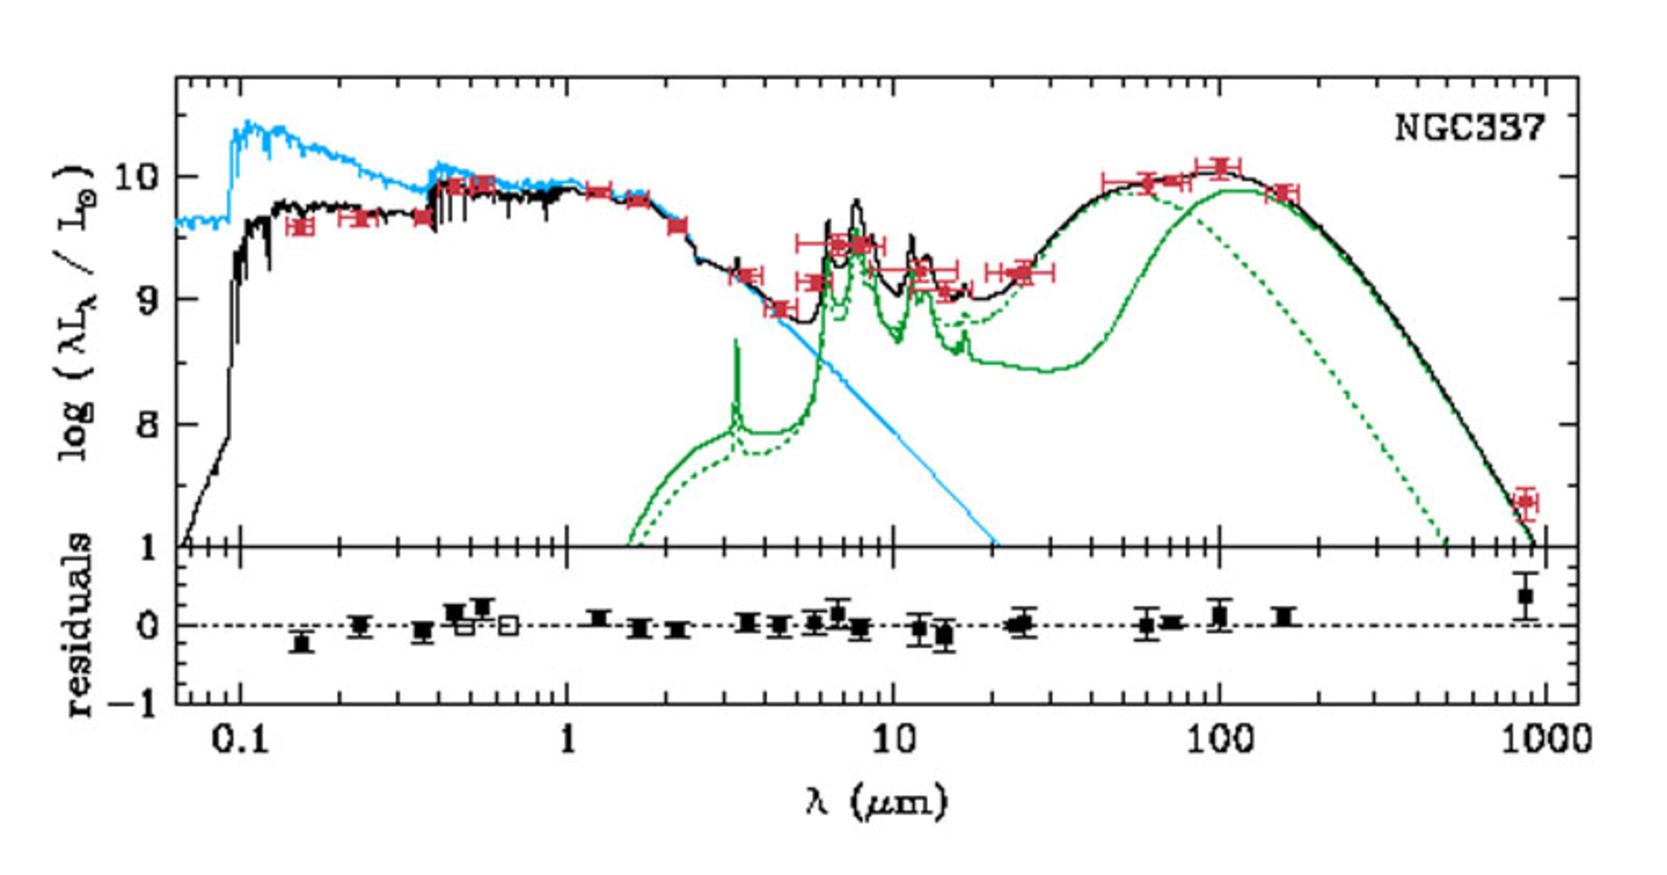
\includegraphics[width=0.9\columnwidth]{Figures/unattenuated_attenuated_sed.pdf}
	\caption{The best fitting SED model to the observed spectra of NGC 337 adapted from \citealt{daCunha_2008}. The blue line represents the unattenuated stellar spectrum and the green lines show the reprocessed light by dust, separated into dust in the diffuse ISM (solid) and dust in molecular clouds (dotted). The attenuated (observed) SED from the UV to far-IR is shown as the black line, which is fitted to the data points (red).}
	\label{fig:unattenuated_attenuated_sed}
\end{figure}

A fundamental assumption that is made throughout this Thesis is that we can trace the hidden star formation in a galaxy via the dust emission observed in the far-IR and sub-mm wavelengths. Figure \ref{fig:interstellar_medium} shows that the dust and gas are well mixed in the ISM of the Galaxy, suggesting that interstellar dust coexists with the gas in the ISM, and is a useful proxy for the star formation activity. Moreover, because most UV emission comes from the star formation activity in a galaxy, the total IR luminosity is often assumed to be directly proportional to the fraction of the energy from star formation that gets absorbed by dust. As a result of these two, the emission from dust is vital in our understanding of the hidden star formation, while the properties of the dust content in galaxies, such as the total mass of dust and its temperature, are useful proxies for the star formation conditions in galaxies.
{\color{red}This paragraph is a little messy, but includes the points that I want. Just tidy it up.}

\subsection{The Lifecycle of Dust}

The lifecycle of dust grains, the mechanisms in which they are produced and destroyed, are important in understanding the metal enrichment and stellar evolution of galaxies. Dust can form in a number of ways including in the stellar winds of evolved stars, from the ejecta of supernovae or they can form in situ in the ISM (\citealt{Draine_2009}). Traditionally, the majority of dust was presumed to be formed in the outer envelopes of latter stage stars, such as red giant branch (RGB) and asymptotic giant branch (AGB) stars. These stars have masses of $1 < M_\textrm{star} [M_\odot] < 8$ and are in a late phase of evolution, having left the (stellar) main sequence and formed heavy elements. The metals solidify into grains in the envelopes of RGB and AGB stars and are carried out in the stellar wind and deposited into the ISM ({\color{red}REFERENCE}). For more massive stars with $M_\textrm{star} > 8\,M_\odot$, dust can form in the ejecta of {\color{red}[...]} supernovae, condensing from the leftover expanding material. The problem with this pathway, however, is that the dust yields from a single supernova are still a matter of debate, with studies observing dust masses in supernova remnants between roughly $0.05\,M_\odot$ and $1\,M_\odot$ (\citealt{Rho_2008}; \citealt{Dunne_2009}; \citealt{Barlow_2010}; \citealt{Matsuura_2011}; \citealt{Gomez_2012}; \citealt{Matsuura_2015}; \citealt{Chawner_2019}). Much of this debate is due to questions about how dust formed in supernovae may survive the destructive shock waves that are produced (\citealt{Draine_1979}; \citealt{Jones_1996}). The production rate of dust is a key open question, particularly for studies in the early Universe where a \textit{Dust Budget Crisis} has been proposed (e.g. \citealt{Dwek_2007}; \citealt{Michalowski_2010}; \citealt{Valiante_2011}). This refers to the difficulty in explaining the high dust masses observed in high redshift galaxies from dust produced via the Low-Intermediate Mass Stars (LIMS). Above redshifts $\sim 5$, there is little time for significant amounts of dust to be produced from the post main-sequence evolution of LIMS (\citealt{Morgan_2003}; \citealt{DiCriscienzo_2013}). The final production mechanism we mention here is dust formed in situ via grain growth. This method is most effective in the dense ISM, and so is particularly important in molecular clouds. Grain growth occurs when the conditions allow for the grains to form mantles of ice, which allow metals to subsequently stick to the grains (coagulation, \citealt{Blain_2004}).

We have mentioned one way in which dust can be destoyed in the ISM, via supernova shocks, but a second process contributing to dust destruction is \textit{sputtering}. Sputtering occurs as the result of the bombardment of gas atoms in dense environments causing the sublimation of the dust grains (\citealt{Barlow_1978}; \citealt{Jones_2004}).

\section{Observing Dusty Star Forming Galaxies in the Far-IR and Sub-mm}

The long wavelengths covering the thermal dust emission can have several names, sometimes referred to as the far-infrared, and at other times as the sub-millimeter. While the two terms are used rather interchangeably, we shall continue with the naming convention that the far-infrared waveband extends from roughly $10$ to $200\,\mu$m, while the sub-millimeter waveband extends from $200\,\mu$m to $1\,$mm. The peak in the dust emission for most galaxies is located at approximately $100\,\mu$m, where the Cosmic Infrared Background (CIB) peaks ({\color{red}REFERENCE}), so in our system the far-IR typically refers to observations that constrain the peak of the spectrum, while sub-mm observations generally constrain the Rayleigh-Jeans side of the SED, for galaxies at $z \lesssim 1$.

The majority of the dust in the ISM by mass has temperatures of roughly {\color{red} $X - X\,$K} ({\color{red}REFERENCES}). It is predominantly the thermal emission from this cold dust that we observe in the far-IR and sub-mm regimes. As can be seen in the example SED of Figure \ref{fig:unattenuated_attenuated_sed}, the dust emission creates a steep sub-mm spectrum. The result of such a steep spectrum in the sub-mm is that we observe a negative \textit{k-correction}. A k-correction is a function of wavelength that is applied to the flux of a redshifted galaxy to convert from the observed frame to the galaxy's rest frame. A strong negative k-correction effectively cancels out the dimming of the flux due to their cosmological distances, meaning that a galaxy of a given IR luminosity will have an approximately constant sub-mm flux at redshifts between $z = 1$ and $z\sim8$ (\citealt{Casey_2014b}). {\color{red}Quick maths calculation, see Casey+2014 Section 2.2 - in reference to long $>850\,\mu$m observations}. The sub-mm regime allows us to access galaxies at earlier epochs where the optical/near-IR wavelengths with positive k-corrections have succumbed to substantial redshift dimming. The galaxies that are detected in this regime are henceforth referred to as Submillimeter Galaxies (SMGs). As we approach the far-IR, climbing up the Rayleigh-Jeans side of the spectrum, the effect of the negative k-correction becomes less strong and the galaxies detected in the far-IR will typically be lower redshift as a result. The benefit here, however, is that at the peak of the dust emission the higher flux density allows us to observe large volumes of local galaxies, even when the sensitivity of the far-IR instrument is sub-optimal. As we shall see, this is used to great effect with far-IR instruments that have surveyed large swathes of sky. The galaxies that are detected from their far-IR emission do not necessarily have their own naming convention (though throughout this Thesis, we heavily refer to \textit{Herschel}-detected galaxies in reference to the far-IR detected galaxies with the \textit{Herschel Space Observatory} which can sometimes be seen referred to as \textit{Herschel}-selected Galaxy, HSG, in the literature). We consider these galaxies under the blanket term of Dusty, Star Forming Galaxies (DSFGs), which, in its vagueness, also encompasses SMGs. All of these galaxies may also be likened to the LIRGs, ULIRGs and HyLIRGs defined earlier, depending on their total IR luminosity.

DSFGs are known to be some of the most massive and extreme examples of star forming galaxies, with star formation rates routinely above $100\,M_\odot$yr$^{-1}$ and stellar masses above $10^{10}\,M_\odot$. The result of having such high star formation rates, these galaxies are highly dust-enshrouded and are reprocessing as much as $95\%$ or more of the emission from young stars to rest frame far-IR (\citealt{Blain_2002}; \citealt{Casey_2014b}). However, as DSFGs are so massive they sit at the tip of the galaxy stellar mass function and are thus rare compared to more "conventional" or "normal" star forming galaxies ({\color{red}REFERENCES}). As a result, many of the DSFGs observed to date have been found in wide area, blind surveys from single-dish far-IR and sub-mm telescopes such as {\color{red}[continue with facilities as mentioned in Casey Astro2020 White Paper]}.

\subsection{The First Submillimeter Galaxies}

The atmospheric transmission of far-IR and sub-mm wavelengths is illustrated in Figure \ref{fig:transmission}. It shows the difficulty in observing electromagnetic radiation in these regimes from the ground, with only select pockets of atmospheric windows allowing for ground-based observations. In the shorter wavelength, far-IR waveband, the transmission is minimal and the idea of a ground-based far-IR instrument is not possible. As we have seen, the dust emission at longer wavelengths in the sub-mm is typically many times fainter, but does allow for a limited number of atmospheric windows, including two important windows at $450\,\mu$m ($670\,$GHz) and $\sim 850\,\mu$m ($350\,$GHz). Making use of these brief windows, the Submillimeter Common User Bolometer Array (SCUBA; \citealt{Holland_1999}) was commissioned on the James Clerk Maxwell Telescope (JCMT) with simulatenous operation at $450-$ and $850\,\mu$m and was soon used to produce the first sub-mm maps (e.g. \citealt{Smail_1997}; \citealt{Barger_1998}; \citealt{Hughes_1998}). These small maps, totalling several square arcminutes, observed a handful of sub-mm bright galaxies that had luminosities much like those of ULIRGs. While sub-mm astronomy was still in its infancy the sample size of SMGs was low, however, these small samples were enough to have important implications on the cosmic star formation history. At the local density of ULIRGs, very few if any such galaxies should have been observed in these fields at $z \gtrsim 1$. The fact that these objects were observed implied a strong evolution in the cosmic star formation history and, while ULIRGs play an insignificant role in the star formation rate density locally, these galaxies formed a substantial contribution ($\gtrsim 10\%$) at high redshifts $z \gtrsim 1$ (\citealt{Casey_2014b}). 

\begin{figure}
    \centering
	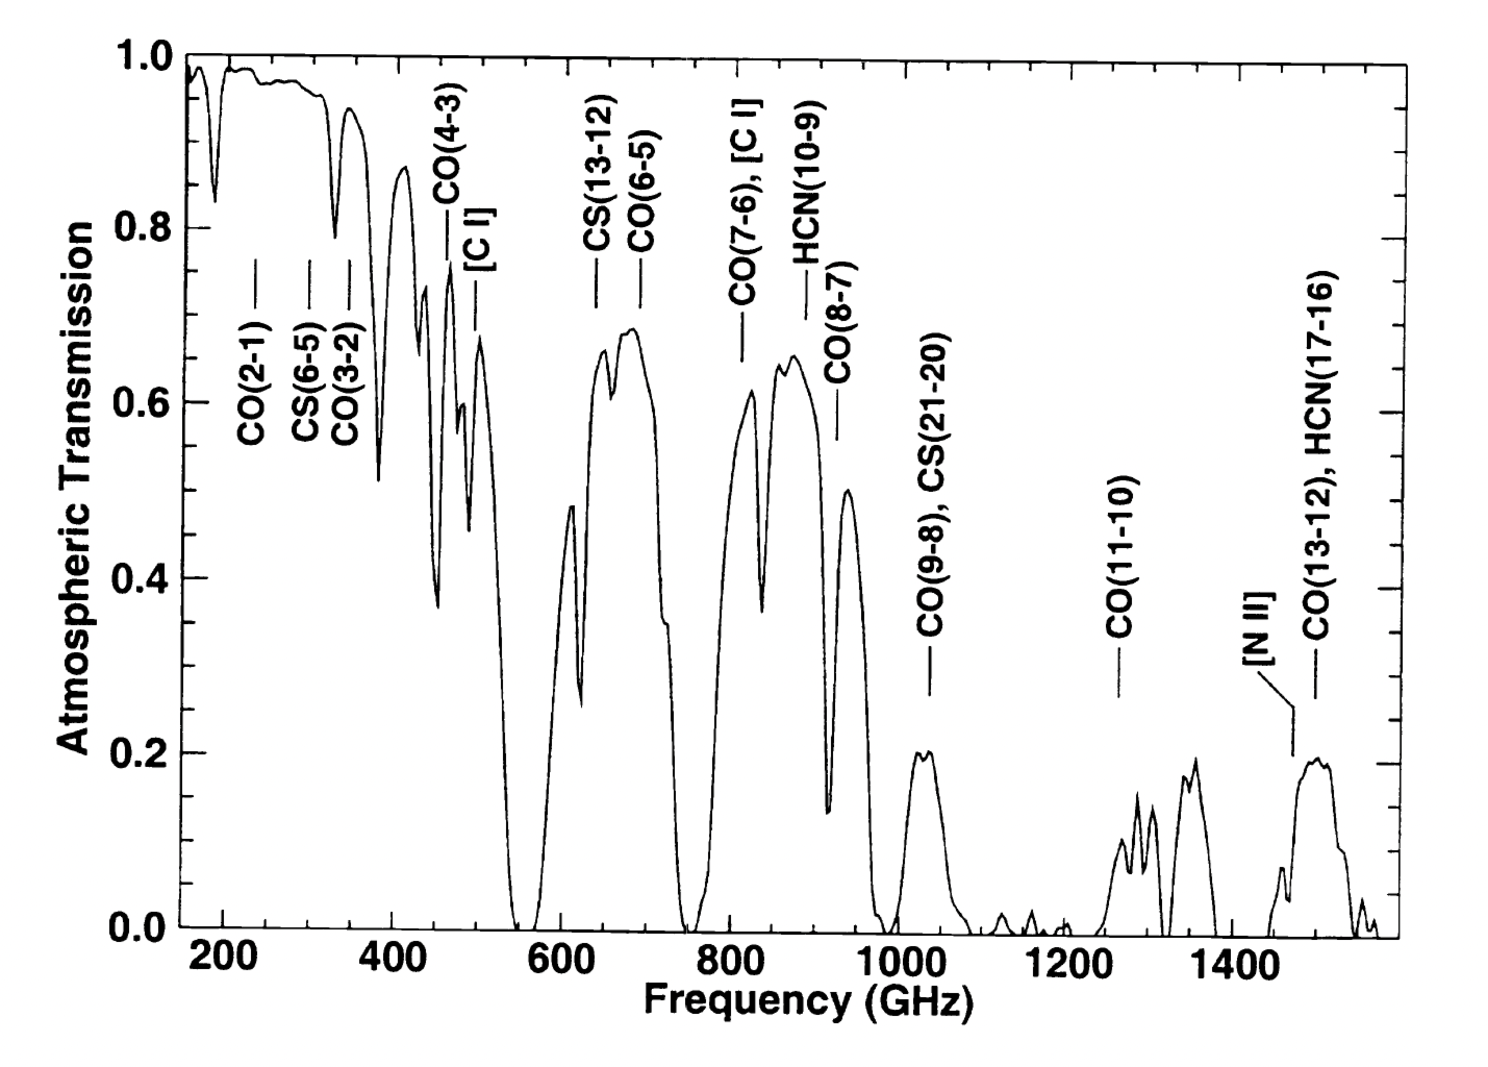
\includegraphics[angle=0.5, width=0.75\columnwidth]{Figures/transmission.pdf}
	\caption{The atmospheric transmission spectrum at (sub-)millimeter wavelengths as observed at Pampa la Bola ($4,800\,$m above sea level in Chile) and illustrated in \citealt{Matsushita_2000}. Overplotted are the locations of various CO, CI, CS, NII and HCN transition lines.}
	\label{fig:transmission}
\end{figure}

Let us briefly return to the Hubble Deep Field, shown in Figure \ref{fig:hubble_deep_field}. We saw that the field contains a wide variety of galaxies with different morphologies, ages and colours. An important point of note is that there are a number of massive ($>10^{10}\,M_\odot$) elliptical galaxies that can be observed in the local Universe. These galaxies are typically characterized by old stellar populations, limited cold gas and dust and red colours. The $z = 0$ ages of these galaxies suggest that they had already formed their stellar mass at high redshift (e.g. \citealt{Gallazzi_2005}; \citealt{Thomas_2005}), implying that at some point in the past, they must have been rapidly forming stars and thus be incredibly bright. Without much luck finding these very active galaxies in the optical, the presence of highly dust-enshrouded galaxies with potentially starbursting phases, provides some credit to the idea that SMGs may be the progenitors of these massive elliptical galaxies in the Universe today, namely \textit{proto-ellipticals} (e.g. \citealt{Toft_2014}; \citealt{Valentino_2020b}). A better understanding of this population of galaxies may be key in our understanding of the obscured star formation at high redshits, and provide a target population in order to study the link between the early and local Universe.

In 1998, SCUBA was used to image the Hubble Deep Field at $450-$ and $850\,\mu$m; the $850\,\mu$m data covering an area of approximately $9$ square arcminutes. At the time, the map of the Hubble Deep Field presented in \citealt{Hughes_1998} was the deepest sub-mm map ever taken - a section covering a radius of $100\,$arcsec from the $850\,\mu$m image center is shown in Figure \ref{fig:hubble_deep_field_scuba}. Much of the peaks in the image are a result of source confusion (Section \ref{sec:challenges}), but $5$ reliable sub-mm sources were identified. Despite a comparatively small number of detections compared to the same size area on the Hubble image, the total energy outputs are roughly the same ({\color{red}REFERENCES}). The brightest source, HDF850.1, is an exceptional example of the extreme nature of these sources. HDF850.1 has a star formation rate of $\sim 850\,M_\odot$yr$^{-1}$ (\citealt{Walter_2012}), which is comparable to the total number of stars we expect to be being formed in all the other galaxies in the optical image combined. Moreover, the incredibly dusty nature of this source means that an unambiguous counterpart at shorter wavelengths could not be identified, even in the deepest optical image of the Universe ever taken at the time. The identification of an optical/infrared counterpart has continued to be elusive with only a handful of studies making claims for having identified the galaxy producing the sub-mm emission, with much contention (e.g. \citealt{Dunlop_2004}; \citealt{Serjeant_2014}; \citealt{Sun_2023}).

\begin{figure}
    \centering
	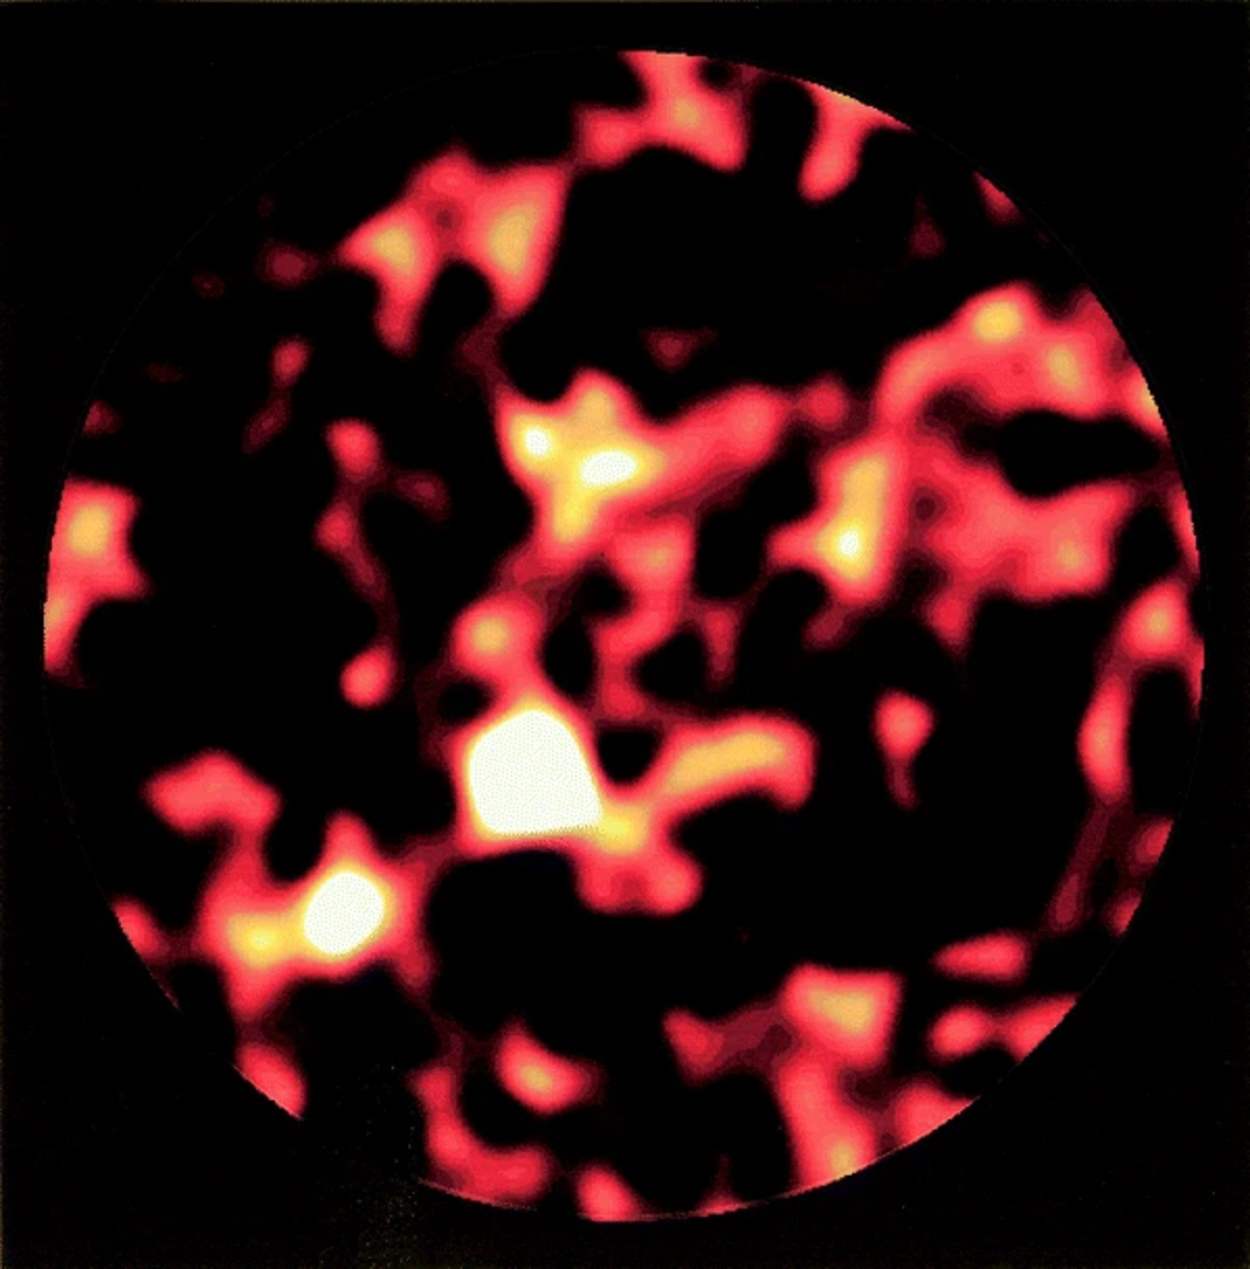
\includegraphics[width=0.75\columnwidth]{Figures/hubble_deep_field_scuba.pdf}
	\caption{The $850\,\mu$m map of the Hubble Deep Field taken with the SCUBA camera on the JCMT and presented in \citealt{Hughes_1998}. The image is of a patch of the field with a radius of $100\,$arcsec and shows $5$ statistically identified sub-mm galaxies.}
	\label{fig:hubble_deep_field_scuba}
\end{figure}

With continual improvement in the sensitvity of bolometer-arrays, samples of DSFGs detected at sub-mm wavelengths, particularly at $\sim 850\,\mu$m, have continually grown (e.g. {\color{red}REFERENCES}). If we wish to observe these same galaxies at far-IR wavelengths closer to the peak of the dust emission we find that the atmospheric transmission falls to zero. These observations are especially vital in characterizing the properties of the dust in these galaxies; without observations constraining the peak of the dust emission basic properties like the mass and temperature of the dust are very hard to predict (as we shall see in Chapter \ref{chapter:Dust_Evolution}).

{\color{red}To observe at far-IR wavelengths (why might you?) then you need to go air-bourne.}

\subsection{The Herschel Space Observatory}

\subsection{Herschel Surveys}

\section{Challenges in Identifying DSFGs and their Multiwavelength Counterparts}
\label{sec:challenges}

\section{Outline of Thesis}

% SOME EXTRAS

%This Thesis focuses on characterizing the dust properties and the evolution in the dust content of these galactic behemoths. 
